\documentclass{beamer}
\usefonttheme{professionalfonts}  % serif math
\setbeamertemplate{frametitle continuation}{} %{(\insertcontinuationcount)}

\iffalse
\usepackage{pgfpages}
\setbeameroption{show notes}
\setbeameroption{show notes on second screen=right}
% pdfpc slajdovi.pdf --notes=right
\fi

%\usepackage[scaled]{beramono}				% sans-serif monospace

%%text%%
	\raggedright						% bez desnog poravnavanja
\raggedbottom
\usepackage{caption}
\captionsetup{%
	justification=raggedright,
}
\usepackage{etoolbox}
\makeatletter
\patchcmd{\@dottedtocline}
{\rightskip\@tocrmarg}
{\rightskip\@tocrmarg plus 4em \hyphenpenalty\@M}
{}{}
\makeatother
\setlength{\parindent}{1em}	 % uvlačenje ulomaka
\usepackage{indentfirst}	 % uvlačenje prvog ulomka
\setlength{\parskip}{0.5em}	 % razmak između ulomaka

\usepackage[multiple, bottom]{footmisc}	 % višestruke fusnote, poslije slika/tablica


\iffalse
\usepackage{xcolor}
\usepackage{color}
\hypersetup{
	colorlinks,
	linkcolor={blue!60!green!50!black},  % xcolor package
	citecolor={green!40!black},
	urlcolor={blue!75!green!30!black}
}
\definecolor{bluekeywords}{rgb}{0.13,0.13,1}  % color package
\definecolor{greencomments}{rgb}{0,0.5,0}
\definecolor{redstrings}{rgb}{0.9,0,0}
\fi



% ULTIMATH


% redefinition of left and right to make spacing consistent
% https://tex.stackexchange.com/questions/2607/spacing-around-left-and-right/2610
\let\originalleft\left
\let\originalright\right
\renewcommand{\left}{\mathopen{}\mathclose\bgroup\originalleft}
\renewcommand{\right}{\aftergroup\egroup\originalright}

\usepackage{amsmath}
\usepackage{amssymb}  % loads amsfonts

% adding equation number inside align*
\newcommand\numberthis{\addtocounter{equation}{1}\tag{\theequation}}

\usepackage{mathtools}  % \coloneqq, smashoperator
%\usepackage{bm}
%\usepackage[utopia]{mathdesign}

%\usepackage{commath}  % calculus, perentheses
% https://tex.stackexchange.com/questions/135944/commath-and-ifinner/135985#135985
% instead of commath:
%% begin commath-fixed
\DeclareMathOperator{\dif}{d\!}
\DeclareMathOperator{\Dif}{D\!}

\makeatletter
\newcommand{\spx}[1]{%
	\if\relax\detokenize{#1}\relax
	\expandafter\@gobble
	\else
	\expandafter\@firstofone
	\fi
	{^{#1}}%
}
\makeatother

\newcommand\pd[3][]{\frac{\partial\spx{#1}#2}{\partial#3\spx{#1}}}
\newcommand\tpd[3][]{\tfrac{\partial\spx{#1}#2}{\partial#3\spx{#1}}}
\newcommand\dpd[3][]{\dfrac{\partial\spx{#1}#2}{\partial#3\spx{#1}}}

\newcommand{\md}[6]{\frac{\partial\spx{#2}#1}{\partial#3\spx{#4}\partial#5\spx{#6}}}
\newcommand{\tmd}[6]{\tfrac{\partial\spx{#2}#1}{\partial#3\spx{#4}\partial#5\spx{#6}}}
\newcommand{\dmd}[6]{\dfrac{\partial\spx{#2}#1}{\partial#3\spx{#4}\partial#5\spx{#6}}}

\newcommand{\od}[3][]{\frac{\dif\spx{#1}#2}{\dif#3\spx{#1}}}
\newcommand{\tod}[3][]{\tfrac{\dif\spx{#1}#2}{\dif#3\spx{#1}}}
\newcommand{\dod}[3][]{\dfrac{\dif\spx{#1}#2}{\dif#3\spx{#1}}}

\newcommand{\genericdel}[4]{%
	\ifcase#3\relax
	\ifx#1.\else#1\fi#4\ifx#2.\else#2\fi\or
	\bigl#1#4\bigr#2\or
	\Bigl#1#4\Bigr#2\or
	\biggl#1#4\biggr#2\or
	\Biggl#1#4\Biggr#2\else
	\left#1#4\right#2\fi
}
\newcommand{\del}[2][-1]{\genericdel(){#1}{#2}}
\newcommand{\cbr}[2][-1]{\genericdel\{\}{#1}{#2}}
\let\set\cbr
\let\event\cbr
\newcommand{\sbr}[2][-1]{\genericdel[]{#1}{#2}}
\newcommand{\intoo}[2][-1]{\mathinner{\genericdel(){#1}{#2}}}
\newcommand{\intcc}[2][-1]{\mathinner{\genericdel[]{#1}{#2}}}
\newcommand{\intoc}[2][-1]{\mathinner{\genericdel(]{#1}{#2}}}
\newcommand{\intco}[2][-1]{\mathinner{\genericdel[){#1}{#2}}}
\newcommand{\eval}[2][-1]{\genericdel.|{#1}{#2}}
\newcommand{\envert}[2][-1]{\genericdel||{#1}{#2}}
\let\abs\envert
\newcommand{\enVert}[2][-1]{\genericdel\|\|{#1}{#2}}
\let\norm\enVert
\newcommand{\fullfunction}[5]{%
	\begin{array}{@{}r@{}l@{}}
		#1 \colon #2 &{}\longrightarrow{}  #3 \\
		#4 &{}\longmapsto{} #5
	\end{array}
}
% parentheses from commath redefined to improve spacing because left and right were redefined, \midmid, new \tilde and \hat that don't make parentheses bigger
\newcommand{\ind}[1]{{\sbr{#1}}}
%% end commath-fixed

\usepackage{stmaryrd}  % \llbracket for \rrbracket, ...

%\newtheorem{definition}{Definicija}[section]
%\newtheorem{theorem}{Teorem}[section]
%\newtheorem{corollary}{Korolar}[theorem]

% More consistent fonts
\usepackage[OMLmathsfit]{isomath}  % \DeclareMathAlphabet ...
\usepackage{upgreek}

\DeclareMathAlphabet{\mathbbmsl}{U}{bbm}{m}{sl}
\DeclareMathAlphabet{\mathbbmb}{U}{bbm}{b}{it}
\DeclareMathAlphabet{\mathbbmssit}{U}{bbmss}{m}{it}

% common set?, distribution
\newcommand{\commset}[1]{\mathbbmb{#1}}
\newcommand{\distrib}[1]{\mathcal{#1}}

% sans-serif blackboard-bold
\newcommand{\mathsfbbit}[1]{\mathbbmssit{#1}}

% variable
\let\vec\relax
\let\set\relax
\newcommand{\vec}[1]{\boldsymbol{#1}}
\newcommand{\set}[1]{\mathbbmsl{#1}}

% constant
\newcommand{\const}[1]{\mathrm{#1}}
\newcommand{\cvec}[1]{\mathbf{#1}}
\newcommand{\cset}[1]{\mathbb{#1}}

% underlining (for random variables)
\newcommand{\nunder}[2][5]{\mathrlap{\mkern\the\numexpr#1/2mu\relax\underline{\phantom{\mathrm{#2}\mkern-#1mu}}}\mathrm{#2}}
\newcommand{\subline}[2][n]{%
    \makebox[\widthof{$#2$}/2]{}\mathclap{#2}%
    \text{\smash{\raisebox{0.04em}{% 0.04
        $\mathclap{\underline{\hphantom{#1}\vphantom{#2}}}$%
    }}}%
    \makebox[\widthof{$#2$}/2]{}%
}

% random variables (Dutch notation - J. Hemelrijk, underlining random variables)
% https://lingpipe-blog.com/2009/10/13/whats-wrong-with-probability-notation/
\newcommand{\rvarstyle}[1]{{{\subline[i]{#1}}}}
\newcommand{\rvar}[1]{\rvarstyle{#1}}
\newcommand{\rvec}[1]{\rvarstyle{\vec{#1}}}
\newcommand{\rset}[1]{\rvarstyle{\set{#1}}}
\newcommand{\var}[1]{{\color{red}#1}}

% linear algebra
\newcommand{\transpose}{\mathsf T}
\newcommand{\tp}{\transpose}

% calculus - commath: od, pd, md, dif
% parentheses - commath: del, cbr, sbr, envert, enVert

% named functions
\DeclareMathOperator{\softplus}{softplus}
\DeclareMathOperator{\softmax}{softmax}
\DeclareMathOperator{\logistic}{\sigma}
\DeclareMathOperator{\sgn}{sgn}
\DeclareMathOperator{\diag}{diag}
\DeclareMathOperator{\ReLU}{ReLU}
\DeclareMathOperator{\modfunc}{mod}

% operators
\DeclareMathOperator{\vecfunc}{vec}
\DeclareMathOperator*{\argmin}{arg\,min} % thin space
\DeclareMathOperator*{\argmax}{arg\,max}
\let\P\relax
\DeclareMathOperator{\P}{P}
\DeclareMathOperator{\p}{\mathrm{p}}
\DeclareMathOperator*{\E}{\mathrm{I\kern-.282em E}}
\DeclareMathOperator*{\D}{\mathrm{I\kern-.282em D}}
\DeclareMathOperator*{\Cov}{\mathrm{Cov}}
%\let\H\relax
\renewcommand{\H}{\mathrm{H}}
\newcommand{\h}{\mathrm{h}}
\newcommand{\I}{\mathrm{I}}
\newcommand{\Dist}{\mathrm{D}}  % D is for dispersion

% graphs
\newcommand{\pa}{\mathrm{pa}}
\newcommand{\ch}{\mathrm{ch}}
\newcommand{\pred}{\mathrm{pred}}
\renewcommand{\succ}{\mathrm{succ}}

% bracket operators
%\newcommand{\enangle}[1]{\mathinner{\left\langle{#1}\right\rangle}}
\newcommand{\enangle}[2][-1]{\genericdel\langle\rangle{#1}{#2}}
\newcommand{\enbbracket}[1]{{\mathinner{\left\llbracket{#1}\right\rrbracket}}}
\newcommand{\braket}[2]{\enangle{{#1}\middle|{#2}}}

%\let\mid\relax
%\newcommand{\mid}{\;|\;}  % spaces around not reduced in index
\newcommand{\midmid}{\;\middle|\;}

% hat and tilde
\let\oldhat\hat
\renewcommand{\hat}[1]{\vphantom{#1}\smash[t]{\oldhat{#1}}}
\let\oldtilde\tilde
\renewcommand{\tilde}[1]{\vphantom{#1}\smash[t]{\oldtilde{#1}}}
%\renewcommand{\tilde}[1]{\stackrel{\sim}{\smash{\mathcal{#1}}\rule{0pt}{1.1ex}}}
%\renewcommand{\tilde}[1]{\overset{\sim}{#1}}}
\let\oldwidetilde\widetilde
\renewcommand{\widetilde}[1]{\vphantom{#1}\smash[t]{\oldwidetilde{#1}}}

% special
%\newcommand{\funcdef}[3]{#1 \in (#2 \to #3)}
\newcommand{\funcdef}[3]{#1 \colon #2 \to #3}
\newcommand{\Dkl}[2]{\Dist_\mathrm{KL}\del{#1\;\middle\|\;#2}}
\newcommand{\C}{\cset{C}}
\newcommand{\R}{\cset{R}}
\newcommand{\Z}{\cset{Z}}
\newcommand{\N}{\cset{N}}
\newcommand{\dirac}{\updelta}

\newcommand\concat{\mathbin{+\mkern-10mu+}}

% machine learning evaluation
\newcommand{\TP}{\mathit{TP}}
\newcommand{\FP}{\mathit{FP}}
\newcommand{\TN}{\mathit{TN}}
\newcommand{\FN}{\mathit{FN}}
\newcommand{\FPR}{\mathit{FPR}}
\newcommand{\TPR}{\mathit{TPR}}
\newcommand{\AUROC}{\mathit{AUROC}}
\newcommand{\AUPR}{\mathit{AUPR}}
\newcommand{\AP}{\mathit{AP}}
\newcommand{\IoU}{\mathit{IoU}}
\newcommand{\mIoU}{\mathit{mIoU}}

% operators and relations
\newcommand{\bidot}{\mkern1.5mu{..}\mkern1.5mu}
%\newcommand\sheq{\mkern1.5mu{=}\mkern1.5mu}
%\renewcommand{\dots}{...}


% no vertical space stretching around display math
\usepackage[nodisplayskipstretch]{setspace}

\newenvironment{talign}
{\let\displaystyle\textstyle\align}
{\endalign}
\newenvironment{talign*}
{\let\displaystyle\textstyle\csname align*\endcsname}
{\endalign}


\usepackage{dashbox}%
%\newcommand\dashedbox[1][H]{\setlength{\fboxsep}{0pt}\setlength{\dashlength}{4pt}\setlength{\dashdash}{2pt} \dbox{\phantom{#1}}}
\newcommand\phbox[1][\phantom{:}]{\setlength{\fboxsep}{0.5pt}\setlength{\dashlength}{4pt}\setlength{\dashdash}{3pt} \raisebox{2pt}{\dbox{$\phantom{:}_{#1}$}}}
%\newcommand\dashedbox[1][H]{\setlength{\fboxsep}{0pt}\dbox{\phantom{#1}}}

\usepackage{booktabs}  % from the template; table quality enhancement

\usepackage{multirow}
\usepackage{tabularx}
%\usepackage{tabu}
%\usepackage{makecell}

%\newcolumntype{P}[1]{>{\raggedright\let\newline\\\arraybackslash\hspace{0pt}}p{#1}}

%\renewcommand{\arraystretch}{1.1}
%\usepackage{floatrow} 				% centriranje svih slika
\usepackage{float}					% figure [H]
\usepackage{graphicx} 				% includegraphics
%\usepackage{caption}			% subfigure
\usepackage{subcaption}			% subfigure
%\usepackage[export]{adjustbox} 	% http://ctan.org/pkg/adjustbox

\usepackage[section]{placeins}  % [section] for \FloatBarrier before every section 

\graphicspath{ {./figures/} }		% mapa sa slikama
%\let\oldincludegraphics\includegraphics
%\renewcommand{\includegraphics}[2][]{\oldincludegraphics[#1,max width=0.9\linewidth]{#2}}

%\usepackage{flafter} % floats after the first reference


\usepackage{relsize}

\usepackage[append]{beamersubframe}  % moving slides to the appendix with subframe instead of frame



% Bibliography
%\usepackage[authoryear]{natbib}
%\usepackage[numbers]{natbib}
\usepackage[backend=bibtex, maxcitenames=2, style=authoryear-comp]{biblatex}
\addbibresource{bibliography}
\renewcommand*{\bibfont}{\scriptsize}

\definecolor{citecolor}{RGB}{24, 128, 24}

\newcommand{\citet}[1]{{\color{citecolor}\relscale{0.8}\textcite{#1}}}
\newcommand{\citep}[1]{{\color{citecolor}\relscale{0.8}[\textcite{#1}]}}



% Beamer

\mode<presentation>
{
	\usetheme{Boadilla}      % or try Darmstadt, Madrid, Warsaw, ...
	\usecolortheme{orchid} % or try albatross, beaver, crane, ...
	\usefonttheme{structurebold}  % or try default, serif, structurebold, ...
	\setbeamertemplate{navigation symbols}{}
	\setbeamertemplate{caption}[numbered]
}
\setbeamercolor{structure}{fg=blue!75!green!80!black}	

%\setbeamertemplate{itemize items}[default]
%\setbeamertemplate{enumerate items}[default]
\setbeamertemplate{section in toc}[circle]
\setbeamertemplate{subsection in toc}[circle]
\setbeamertemplate{items}[circle]
\setbeamertemplate{blocks}[default]
\setbeamertemplate{footline}
{
	\leavevmode%
	\hbox{%
		\begin{beamercolorbox}[wd=.15\paperwidth,ht=2.25ex,dp=1ex,center]{author in head/foot}%
			%\usebeamerfont{author in head/foot}\insertshortauthor
		\end{beamercolorbox}%
		\begin{beamercolorbox}[wd=.7\paperwidth,ht=2.25ex,dp=1ex,center]{author in head/foot}%
			\usebeamerfont{title in head/foot}\insertshorttitle  %\hspace*{3em}
		\end{beamercolorbox}%
		\begin{beamercolorbox}[wd=.15\paperwidth,ht=2.25ex,dp=1ex,right]{author in head/foot}%
			\insertframenumber{} / \inserttotalframenumber\hspace*{1ex}
		\end{beamercolorbox}
	}%
	\vskip0pt%
}

\iftrue
\AtBeginSection[]
{
	\begin{frame}<beamer>
		\frametitle{Outline}
		\tableofcontents[currentsection]
	\end{frame}
}
\fi






\title{Interplay of adversarial robustness and generalization in deep convolutional models}
\author{Ivan Grubi\v si\'c \newline \emph{Mentor:} Sini\v sa \v Segvi\'c}
\institute{Faculty of Electrical Engineering and Computing\\
Department of Electronics, Microelectronics, Computer and Intelligent Systems}
\date{}



\begin{document}
	
\begin{frame}
  \titlepage
\end{frame}

\begin{frame}{Content}
  \tableofcontents
\end{frame}


\section{Nonrobustness of machine learning algorithms}

\begin{frame}[allowframebreaks=0.9]{Nonrobustness of machine learning algorithms}
	\begin{itemize}
		\item Current state-of-the-art machine learning algorithms do not work well with \textbf{domain-shifted, out-of-distribution and inputs crafted to fool them} and they often make \textbf{overconfident predictions} \citep{Hendrycks:2016:BDMOODE,Ganin:2015:UDAB,Nguyen:2015:DNNEFHCPUI,Hendrycks:2019:BNNRCCP,Engstrom:2017:RTSFCST,Szegedy:2013:IPNN}.
		\item It is even possible to slightly, even impreceptibly, modify an input (e.g. image) to generate an adversarial example and cause a misprediction.
		\item This is not limited to complex deep models		
		\item This indicates that current algorithms \textbf{perform well without actually understanding data} (in a way similar to humans).
	\end{itemize}
\end{frame}
\note[itemize]{\item\item 0:40 / 0:40}

\begin{frame}[allowframebreaks=0.9]{Nonrobustness of machine learning algorithms}
	\begin{itemize}
		\item A single small gradient descent step on an image increasing the loss is often enough to fool a classifier \citep{Goodfellow:2014:EHAE}.
		\item Sometimes a single pixel can change the prediction \citep{Su:2017:OPAFDNN}.
	\end{itemize}
	\begin{figure}
	\centering
	{\scriptsize
		\begin{tabular}{>{\centering\arraybackslash}m{.22\columnwidth}m{.1in}>{\centering\arraybackslash}m{.22\columnwidth}m{.05in}>{\centering\arraybackslash}m{.22\columnwidth}}
			\centering\arraybackslash
			%abs max for panda was 138, eps was 1., so relative eps is ~.007
			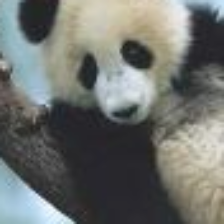
\includegraphics[width=.22\columnwidth]{adversarial-examples/panda_577.png} &%
			\centering\arraybackslash%
			$\centering +\ \epsilon \cdot$ &%
			
\includegraphics[width=.22\columnwidth]{adversarial-examples/nematode_082.png} &%
			$\centering =$ & %
			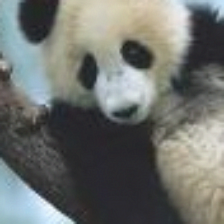
\includegraphics[width=.22\columnwidth]{adversarial-examples/gibbon_993.png} \\
			$\centering \vec x$     &%
			& $\sgn\del{\nabla_{\vec x} L(y,h(\vec x))}$ & & $\tilde{\vec x}$ \\
			\emph{panda} (0.577) & & & & \emph{gibbon} (0.993) 
		\end{tabular}
	}
	\caption{Generation of an adversarial example with FGSM, a single step attack. Italic words and numbers represent classes and confidences. The images are from \citet{Goodfellow:2014:EHAE}.}
	\label{fig:fgsm-adversarial-example}
	\end{figure}
\end{frame}
\note[itemize]{\item\item 0:20 / 1:00}

\begin{frame}{Adversarial robustness and generalization}
	\begin{itemize}
		\item Evidence suggests that there is a \textbf{trade-off between robustness and generalization} with current algorithms \citep{Tsipras:2018:RMBOA,Madry:2017:TDLMRAA,Su:2018:IRTCOACSRDICM}.
		\item The trade-off is \textbf{counter-intuitive} because \textbf{a hypothesis which optimally generalizes would have no adversarial examples} (and an optimal hypothesis exists given a data distribution).
		\item The question remains whether it is achievable regarding computational and data limitations to implement such algorithms.
	\end{itemize}
\end{frame}
\note[itemize]{\item\item 0:40 / 1:40}

\section{Adversarial example definitions}

\begin{subframe}[allowframebreaks=0.9]{Adversarial example definitions}
	\begin{itemize}
		\item A common but imprecise definition of an adversarial example is \textit{an input designed to fool a hypothesis into producing a misprediction}.
		\item Some broader definitions also consider \textbf{out-of-distribution} examples \citep{Gal:2018:SCIMHNAETESBNN} or \textbf{any} inputs that fools the hypothesis \citep{Brown:2018:UAE}, but those will be not considered.
	\end{itemize}
\end{subframe}
% subframe

\begin{frame}[allowframebreaks=0.9]{Adversarial example definitions}
	\begin{definition}[practical adversarial example] \label{def:ae-practical}
		A practical adversarial example is an input for which the following holds:
		\begin{enumerate}
			\item It is \textbf{close} to an input $\vec x$ with a correct prediction.
			\item The \textbf{hypothesis} produces a \textbf{different prediction} than for $\vec x$.
		\end{enumerate}
	\end{definition}
	\begin{definition}[adversarial example] \label{def:ae-consistent}
	An adversarial example is an input for which the following holds:
	\begin{enumerate}
		\item It is \textbf{close} to an input with a correct prediction.
		\item The \textbf{hypothesis} produces a \textbf{misprediction}.
	\end{enumerate}
\end{definition}
\end{frame}
\note[itemize]{\item\item 2:00 / 4:20}

\begin{frame}[allowframebreaks=0.9]{Adversarial example definitions}
	\begin{itemize}
	\item The set of adversarial examples is a function of the \textbf{hypothesis}, a \textbf{neighbourhood function}, the \textbf{input data distribution}, and either
	\begin{itemize}
		\item a reference \textbf{input} (first definition) or
		\item the \textbf{true hypothesis} (second definition).
	\end{itemize}
	\item The practical definition is
	\begin{itemize}
		\item \textbf{inconsistent} -- examples close to class boundaries can be both adversarial and correctly classified depending on the reference, and 
		\item \textbf{practical for generating adversarial examples and robustnes evaluation}.
	\end{itemize}
	\item The second definition is 
	\begin{itemize}
		\item \textbf{impractical} -- it requires knowing the true hypothesis,
		\item \textbf{consistent} -- the true hypothesis has no adversarial examples, and 
		\item \textbf{helpful for achieving the goal of both robustness and generalization}.
	\end{itemize}
\end{itemize}
\end{frame}
\note[itemize]{\item\item 3:00 / 7:20}

\section{Properties of adversarial examples}

\begin{frame}[allowframebreaks=0.9]{Properties of adversarial examples}
\begin{itemize}
	\item Adversarial examples are \textbf{close to clean inputs and rare}, i.e. hard to find by randomly sampling the $L^p$ neighbourhood \citep{Szegedy:2013:IPNN}.    
	\item The neighbourhood of an input contains adversarial examples classified in different classes, i.e. an input is \textbf{close to many class boundaries} of the learned hypothesis.
    \item Knowing the locally \textbf{linear} behaviour of the hypothesis is often enough to generate an adversarial example \citep{Goodfellow:2014:EHAE}.
    \item Adversarial examples \textbf{generalize across algorithms and datasets}, i.e. an adversarial example of one model is often also an adversarial example of some other trained model \citep{Szegedy:2013:IPNN,Papernot:2016:TMLPBBAAS,Liu:2016:DTAEBBA,Tramer:2017:STAE}.
\end{itemize}
\end{frame}
\note[itemize]{\item\item 0:40 / 9:00}

\begin{frame}[allowframebreaks=0.9]{Properties of adversarial examples}
\begin{itemize}
    \item \citet{Tanay:2016:ABTPPAE} hypothesize that adversarial examples might be occurring along \textbf{low-variance directions of the data} and that robustness could be improved with regularization.
    \item \citet{Gilmer:2018:AS} hypothesize that the existence of adversarial examples could be a naturally occurring result of the \textbf{geometry of high-dimensional data manifolds}.
    \item \citet{Tsipras:2018:RMBOA,Ilyas:2019:AENBTF} hypothesize that adversarial examples exist because classifiers rely on \textbf{highly predictive but brittle (nonrobust) features}. \citet{Ilyas:2019:AENBTF} provide good evidence.
\end{itemize}
\end{frame}
\note[itemize]{\item\item 1:00 / 10:00}

\begin{frame}[allowframebreaks=0.9]{Properties of adversarial examples}
\begin{itemize}
    \item (Some) generative models are also vulnerable to adversarial attacks as well \citep{Kos:2018:AEGM, Goodfellow:2014:EHAE}. Figure \ref{fig:vae-gan-targetad-face} shows adversarial examples on a VAE-GAN.
\end{itemize}
\begin{figure}[htbp!]
	\begin{center}
		\raisebox{-0.5\height}{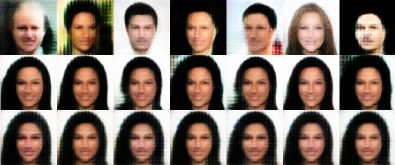
\includegraphics[scale=0.7]{figures/adversarial-examples/kos-exp11-faces-summary.png}}
		~
		\raisebox{-0.5\height}{
\includegraphics[scale=0.075]{figures/adversarial-examples/kos-exp11-faces-target-reconstruction.png}}
	\end{center}
	\caption{Reconstruction outputs for targeted attacks on a VAE-GAN from \citet{Kos:2018:AEGM}. Rows represent reconstructions of original images (top), adversarial examples generated using an attack in latent space (middle) and a VAE-loss attack (bottom). The target reconstruction is on the right.}
	\label{fig:vae-gan-targetad-face}
\end{figure}
\end{frame}
\note[itemize]{\item\item 0:30 / 10:30}

\begin{frame}[allowframebreaks=0.9]{Properties of adversarial examples}
\begin{itemize}
    \item Adversarial examples of \textbf{robust classifiers} are truly \textbf{ambigous} to humans \citep{Tsipras:2018:RMBOA,Li:2019:AGCMRAA}, which suggests that they \textbf{understand data} much better. The semantic meaningfulness of adversarial examples of robust hypotheses is illustrated in figures \ref{fig:tsipras-robust-adversarial-examples}, \ref{fig:rony-cifar10-cherry-picked}, and \ref{fig:li-gfz-adversarial-examples-mnist}.
\end{itemize}
\begin{figure}
	\begin{center}
		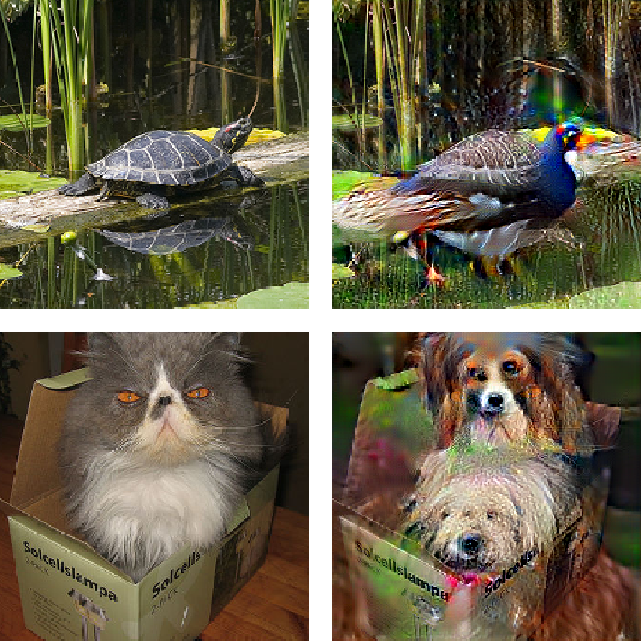
\includegraphics[width=0.5\columnwidth]{figures/adversarial-examples/tsipras-turtle-bird-cat-dogs}
	\end{center}
	\caption{Cherry-picked original images and adversarial examples generated with a large perturbation using an iterative non-targeted attack on an adversarially trained Restricted ImageNet classifier from \citet{Tsipras:2018:RMBOA}.}
	\label{fig:tsipras-robust-adversarial-examples}
\end{figure}

\begin{figure}
	\begin{center}
		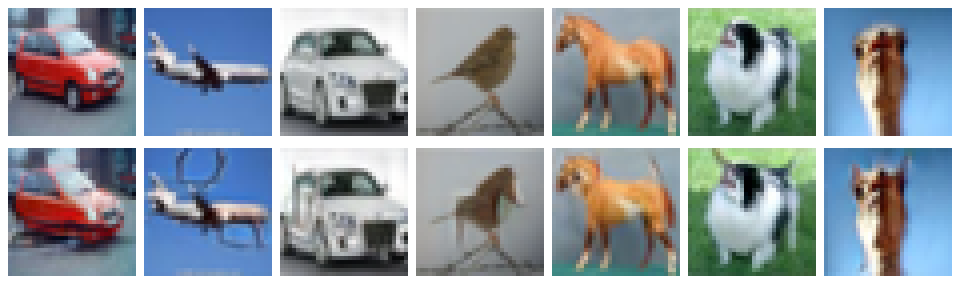
\includegraphics[width=\textwidth]{figures/adversarial-examples/rony/cifar10_cherry_picked}
	\end{center}
	\caption{Cherry-picked clean images (top) and adversarial examples (bottom) generated using an iterative $L^2$-bounded attack on a CIFAR-10 classifier. The predicted classes for the bottom row are \textit{ship},\textit{deer},\textit{truck},\textit{horse},\textit{dog},\textit{cat},\textit{cat}. Adapted from \citep{Rony:2018:DDNEGBLAAD}.}
	\label{fig:rony-cifar10-cherry-picked}
\end{figure}

\begin{figure}
	\begin{center}
		\raisebox{-0.5\height}{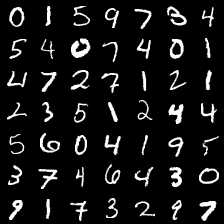
\includegraphics[scale=0.7]{figures/adversarial-examples/li-data_clean.png}}
		\
		\raisebox{-0.5\height}{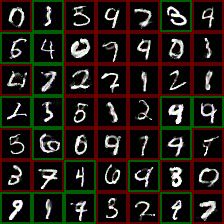
\includegraphics[scale=0.7]{figures/adversarial-examples/li-bayes_A_cw_adv.png}}
	\end{center}
	\caption{Clean images (left) and adversarial examples generated using an iterative non-targeted attack on a generative MNIST classifier with the factorization $\p(\vec z)\p(\vec y\mid\vec z)\p(\vec x\mid\vec z,\vec y)$ (right) from \citet{Li:2019:AGCMRAA}. The adversarial examples marked in green are successful.}
	\label{fig:li-gfz-adversarial-examples-mnist}
\end{figure}
\end{frame}
\note[itemize]{\item\item 1:30 / 12:00}


\section{Attacks and defenses}

\begin{frame}[allowframebreaks=0.9]{Finding adversarial examples}
\begin{itemize}
	\item Let $\set X$ be the input space,
	and $d\in(\set X\times\set X\to \R^+)$ a \textbf{distance function}. The \textbf{neighbourhood} of an example $\vec x$ can be $B_{\epsilon}(\vec x) = \cbr{\vec x'\colon d(\vec x', \vec x) \leq \epsilon}$,
	where $\epsilon$ is the maximum distance.
	
	\item Ideally, the neighbourhood of an example $\vec x$ should be the set of \textbf{perceptually similar} examples that all belong to the same class as $\vec x$, but it requires knowing the true hypothesis.
	\item A common choice for distance $d$ is $L^p$ distance with $p\in\cbr{1,2,\infty}$.
	
	\item Finding an adversarial example can be defined as a constrained optimization problem of \textbf{maximizing some loss with respect to the input} with a constraint of a neighbourhood $B_\epsilon(\vec x)$:
	\begin{align}
	\tilde{\vec x} = \argmax_{\vec x'\in B_\epsilon(\vec x)} L(y, h(\vec x')) \text{,} \label{eq:non-targeted-loss-attack}
	\end{align}
	where $y$ is the true label, $h$ the hypothesis, and $L$ the loss function. 
	\item An objective can also be to find \textbf{the closest adversarial example} \citep{Moosavi-Dezfooli:2016:DFSAMFDNN}:
	\begin{align}
	\tilde{\vec x} = \argmin_{\vec x'\colon \vec x'\in B_\epsilon(\vec x) \land \hat{h}(\vec x') \neq y} d(\vec x', \vec x) \text{,} \label{eq:non-targeted-closest-attack}
	\end{align}
	where $\hat{h}(\vec x) \coloneqq \argmax_{y} h(\vec x)_\ind{y}$.
	\item There are also \textbf{targeted attacks}, where the objective is to get an adversarial example that is classified to some target class. Targeted attack objectives corresponding to equations \eqref{eq:non-targeted-loss-attack} and \eqref{eq:non-targeted-closest-attack} are:
	\begin{align}
	\tilde{\vec x} &= \argmin_{\vec x'\in B_\epsilon(\vec x)} L(y_\text{a}, h(\vec x')) \text{,} \label{eq:targeted-loss-attack} \\
	\tilde{\vec x} &= \argmin_{\vec x'\colon \vec x'\in B_\epsilon(\vec x) \land \hat{h}(\vec x') = y_\text{a}} d(\vec x', \vec x) \text{,} \label{eq:targeted-closest-attack}
	\end{align}
	where $y_\text{a}$ denotes the adversarial target label. 
\end{itemize}
\end{frame}
\note[itemize]{\item\item 1:20 / 13:20}

\begin{frame}[allowframebreaks=0.9]{Finding adversarial examples}
\begin{itemize}
	\item Non-targeted adversarial examples can also be generated by using the prediction instead of the true label in the loss, resulting in \textbf{virtual adversarial examples}.	
	\item \citet{Miyato:2017:VATRMSSSL,Kurakin:2016:AMLS} propose the following attack objective for use in semi-supervised learning:
	\begin{align}
	\tilde{\vec x} = \argmin_{\vec x'\in B_\epsilon(\vec x)} D((\rvar y\mid \vec x, \vec\theta), (\rvar y\mid \rvec x = \vec x', \vec\theta)) \text{,}
	\end{align}
	where $D$ is some distribution distance function.
\end{itemize}
\end{frame}
\note[itemize]{\item\item 1:20 / 13:20}

\begin{frame}[allowframebreaks=0.9]{Common attacks}
	\begin{itemize}
		\item General constrained optimization algorithms as well as more specific ones can be used to generate adversarial examples.
		\item Some common atacks are:
		\begin{itemize}
			\item Box-constrained L-BFGS -- \citet{Szegedy:2013:IPNN} propose to minimize $c\enVert{\vec x -\tilde{\vec x}}_2^2+L(y,h(\tilde{\vec x}))$ with the constraint $\tilde{\vec x}\in\intcc{0,1}$ with L-BFGS, a quasi-Newton optimization method.
			\item Fast gradient sign method (FGSM) -- an attack proposed by \citet{Goodfellow:2014:EHAE} that requires a single gradient computation:
			\begin{align}
			\tilde{\vec x} = \vec x + \epsilon\nabla_{\vec x} L(y,h(\vec x)) \text{.}
			\end{align} 
			%\item DeepFool -- an iterative non-targeted attack proposed by \citet{Moosavi-Dezfooli:2016:DFSAMFDNN} that in each step finds the optimal solution to a linear approximation of a loss in the $L^2$ ball $B_\epsilon(\vec x)$ using the gradient in the current adversarial input. It is faster and finds smaller perturbations than L-BFGS and stronger than FGSM.
			\item Projected gradient descent (PGD) \citep{Madry:2017:TDLMRAA}\footnote[frame]{Equialent to BIM \citep{Kurakin:2016:AMLS} up to random initialization.} -- an iterative gradient-based algorithm with random initialization \citep{Madry:2017:TDLMRAA} of the perturbation from within $B_\epsilon(\vec x)$ at the start and steps in the direction of the gradient sign:
			\begin{equation} \label{eq:pgd}
			\tilde{\vec x}_i = \Pi_{B_\epsilon(\vec x)} \del{\tilde{\vec x}_{i-1} + \alpha\sgn\del{\nabla_{\tilde{\vec x}_{i-1}} L(y,h(\tilde{\vec x}_{i-1}))}} \text{.}
			\end{equation}
			$\alpha$ is the step size, $\Pi_{B_\epsilon(\vec x)}$ is the projection into the $L^p$ $\epsilon$-ball around $\vec x$.
			\item Carlini-Wagner (CW) attacks -- \citet{Carlini:2017:TERNN} propose attacks with similar minimal perturbation objectives as \citet{Szegedy:2013:IPNN} 
			%and \citet{Moosavi-Dezfooli:2016:DFSAMFDNN}
			. They modify the loss and they introduce change of variables $\vec\delta=\frac{1}{2}\del{\tanh\del{\vec w} + \cvec 1} - \vec x$ to limit the perturbation $\vec\delta$ to $\intcc{0,1}$. 
		\end{itemize}
		\item The CW and PGD attacks are currently some of the strongest attacks, suitable for robustness evaluation.		
	\end{itemize}
\end{frame}

\begin{frame}[allowframebreaks=0.9]{Improving adversarial robustness}
	\begin{itemize}
		\item There are different defenses, most of which have been shown to be nonrobust, but had appeared robust because of deficiencies in robustness evaluation  \citep{Carlini:2017:AEANEDBTM,Athalye:2018:OGGFSS,Uesato:2018:ARDEAWA,Carlini:2017:TERNN}.
		\item Some approaches use \textbf{generative models} to approximately \textbf{project inputs to a learned data manifold} (e.g. \citet{Samangouei:2018:DGPCAAAUGM})
		\item Some are based on \textbf{limiting the Lipschitz constant} of the model to limit sensitivity to small input perturbations by regularization and model modification (e.g. \citet{Qian:2018:L2NNN}), some research is looking into ways of \textbf{guaranteeing robustness} (e.g. \citet{Cohen:2019:CARRS}).
		\item The defense currently believed to be most effective according to \citet{Athalye:2018:OGGFSS} is \textbf{adversarial training} \citep{Goodfellow:2014:EHAE} with a strong iterative attack \citep{Madry:2017:TDLMRAA}.
	\end{itemize}
\end{frame}

\begin{frame}[allowframebreaks=0.9]{Adversarial training and empirical
		adversarial risk}
	\begin{itemize}	
		\item \citet{Madry:2017:TDLMRAA} define what can be called \textbf{empirical adversarial risk} by allowing the worst-case attack to modify each input:
		\begin{align}
		R_\text{EA}(h,\set D) \coloneqq \E_{(\vec x, y)\sim p_{\set D}} \del{\max_{\tilde{\vec x}\in B_\epsilon(\vec x)} L(y,h(\tilde{\vec x}))} \text{.}
		\end{align}
		\item They propose PGD for the attack during training and PGD with many iterations to get a better upper bound on robustness. 
		
		\item Adversarially trained models are \textbf{not robust to stronger attacks} than those used for training \citep{Schott:2018:TDFARNNMM}. 
		Because of generating adversarial examples using non-ideal $L^p$ distance, \textbf{performance is affected} \citep{Madry:2017:TDLMRAA,Tsipras:2018:RMBOA} and there can exist \textbf{invariance-based adversarial examples} \citep{Jacobsen:2019:EEICNBAR}.
	\end{itemize}
\end{frame}

\begin{subframe}[allowframebreaks=0.9]{Robustness evaluation}
	\begin{itemize}
		\item For adversarial training with weaker attacks, non-targeted attacks should be preferred due to \textbf{label leaking} \citep{Kurakin:2016:AMLS} where the learned classifier can overfit to adversarial examples and perform better on them than on natural examples, especially with attacks with a small number of iterations. 
		\item For robustness evaluation with datasets that have many similar classes, non-targeted attacks can too easily fool the classifier and targeted attacks give more meaningful evaluation results \citep{Athalye:2018:OGGFSS}.
	\end{itemize}
\end{subframe}

\section{Adversarial robustness and generalization} \label{sec:robustness-generalization}

\begin{frame}[allowframebreaks=0.9]{A trade-off between robustness and generalization}
	\begin{itemize}
		\item \citet{Madry:2017:TDLMRAA,Su:2017:OPAFDNN,Tsipras:2018:RMBOA} and others have empirically observed that adversarial robustness with current algorithms requires \textbf{more capacity} and \textbf{negatively affects generalization}. 
		\item \citet{Su:2017:OPAFDNN} observe that older convolutional architectures with no shortcut connections
		%, like AlexNet \citep{Krizhevsky:2012:ICDCNN} and VGG \citep{Simonyan:2014:VDCNLSIR} 
		seem to be inherently more robust than better performing architectures
		% like ResNet \citep{He:2015:DRLIR}, DenseNet \citep{Huang:2016:DCCN}, MobileNet \citep{Howard:2017:MECNNMVA} and NASNets \citep{Zoph:2018:LTASIR} 
		with standard training.
		\item \citet{Tsipras:2018:RMBOA}, based on the practical definition of an adversarial example, theoretically demonstrate an aspect of the trade-off. 
		\item Another cause of performance drop suggested by them is that salient features might be \textbf{harder to learn} and that algorithms rely on \textbf{highly predictive but nonrobust} features.
	\end{itemize}
\end{frame}
\note[itemize]{
	\item\item 0:20 / 10:20
}

\begin{frame}[allowframebreaks=0.9]{Nonrobust features}
	\begin{itemize}
		%\item Based on some ideas from \citet{Tsipras:2018:RMBOA},  \citet{Ilyas:2019:AENBTF} propose an interesting and experimentally well supported hypothesis on properties features that well-generalizing nonrobust classifiers learn. 
		%\item They show that existence of adversarial examples can be directly attributed to existence of \textbf{nonrobust features}, "features derived from patterns in the data that are \textbf{highly predictive} but \textbf{brittle and incomprehensible to humans}"
		\item \citet{Ilyas:2019:AENBTF} give good experimental support for the hypothesis on reliance on highly-predictive nonrobust features.
		\item In one experiment, they
		\begin{enumerate}
			\item construct a training set $\set D_\text{NR}$ where the only \textbf{useful features are nonrobust features} by generating \textbf{adversarial examples} for a standardly trained classifier and \textbf{relabeling} them with target labels,
			\item \textbf{train a new classifier on the nonrobust dataset} $\set D_\text{NR}$,
			\item test the new classifier on the original test set, where it achieves \textbf{performance close to the original classifier} and \textbf{lower robustness}.
		\end{enumerate}		
		\item In another experiment, they
		\begin{enumerate}
			\item construct a training set $\set D_\text{R}$ with removed \textbf{nonrobust features} using a robust classifier,
			\item \textbf{train a new classifier on the robust dataset} $\set D_\text{R}$,
			\item test the new classifier on the original test set, where it achieves a bit \textbf{lower performance} and \textbf{significantly higher robustness}.
		\end{enumerate}
		%\item Results of these experiments with the CIFAR-10 dataset \citep{Krizhevsky:2009:LMLFTI} are shown in figure \ref{fig:iliyas-experiment-results}.
	\end{itemize}
	\begin{figure}
		\centering
		\begin{subfigure}[b]{0.49\textwidth}
			\centering
			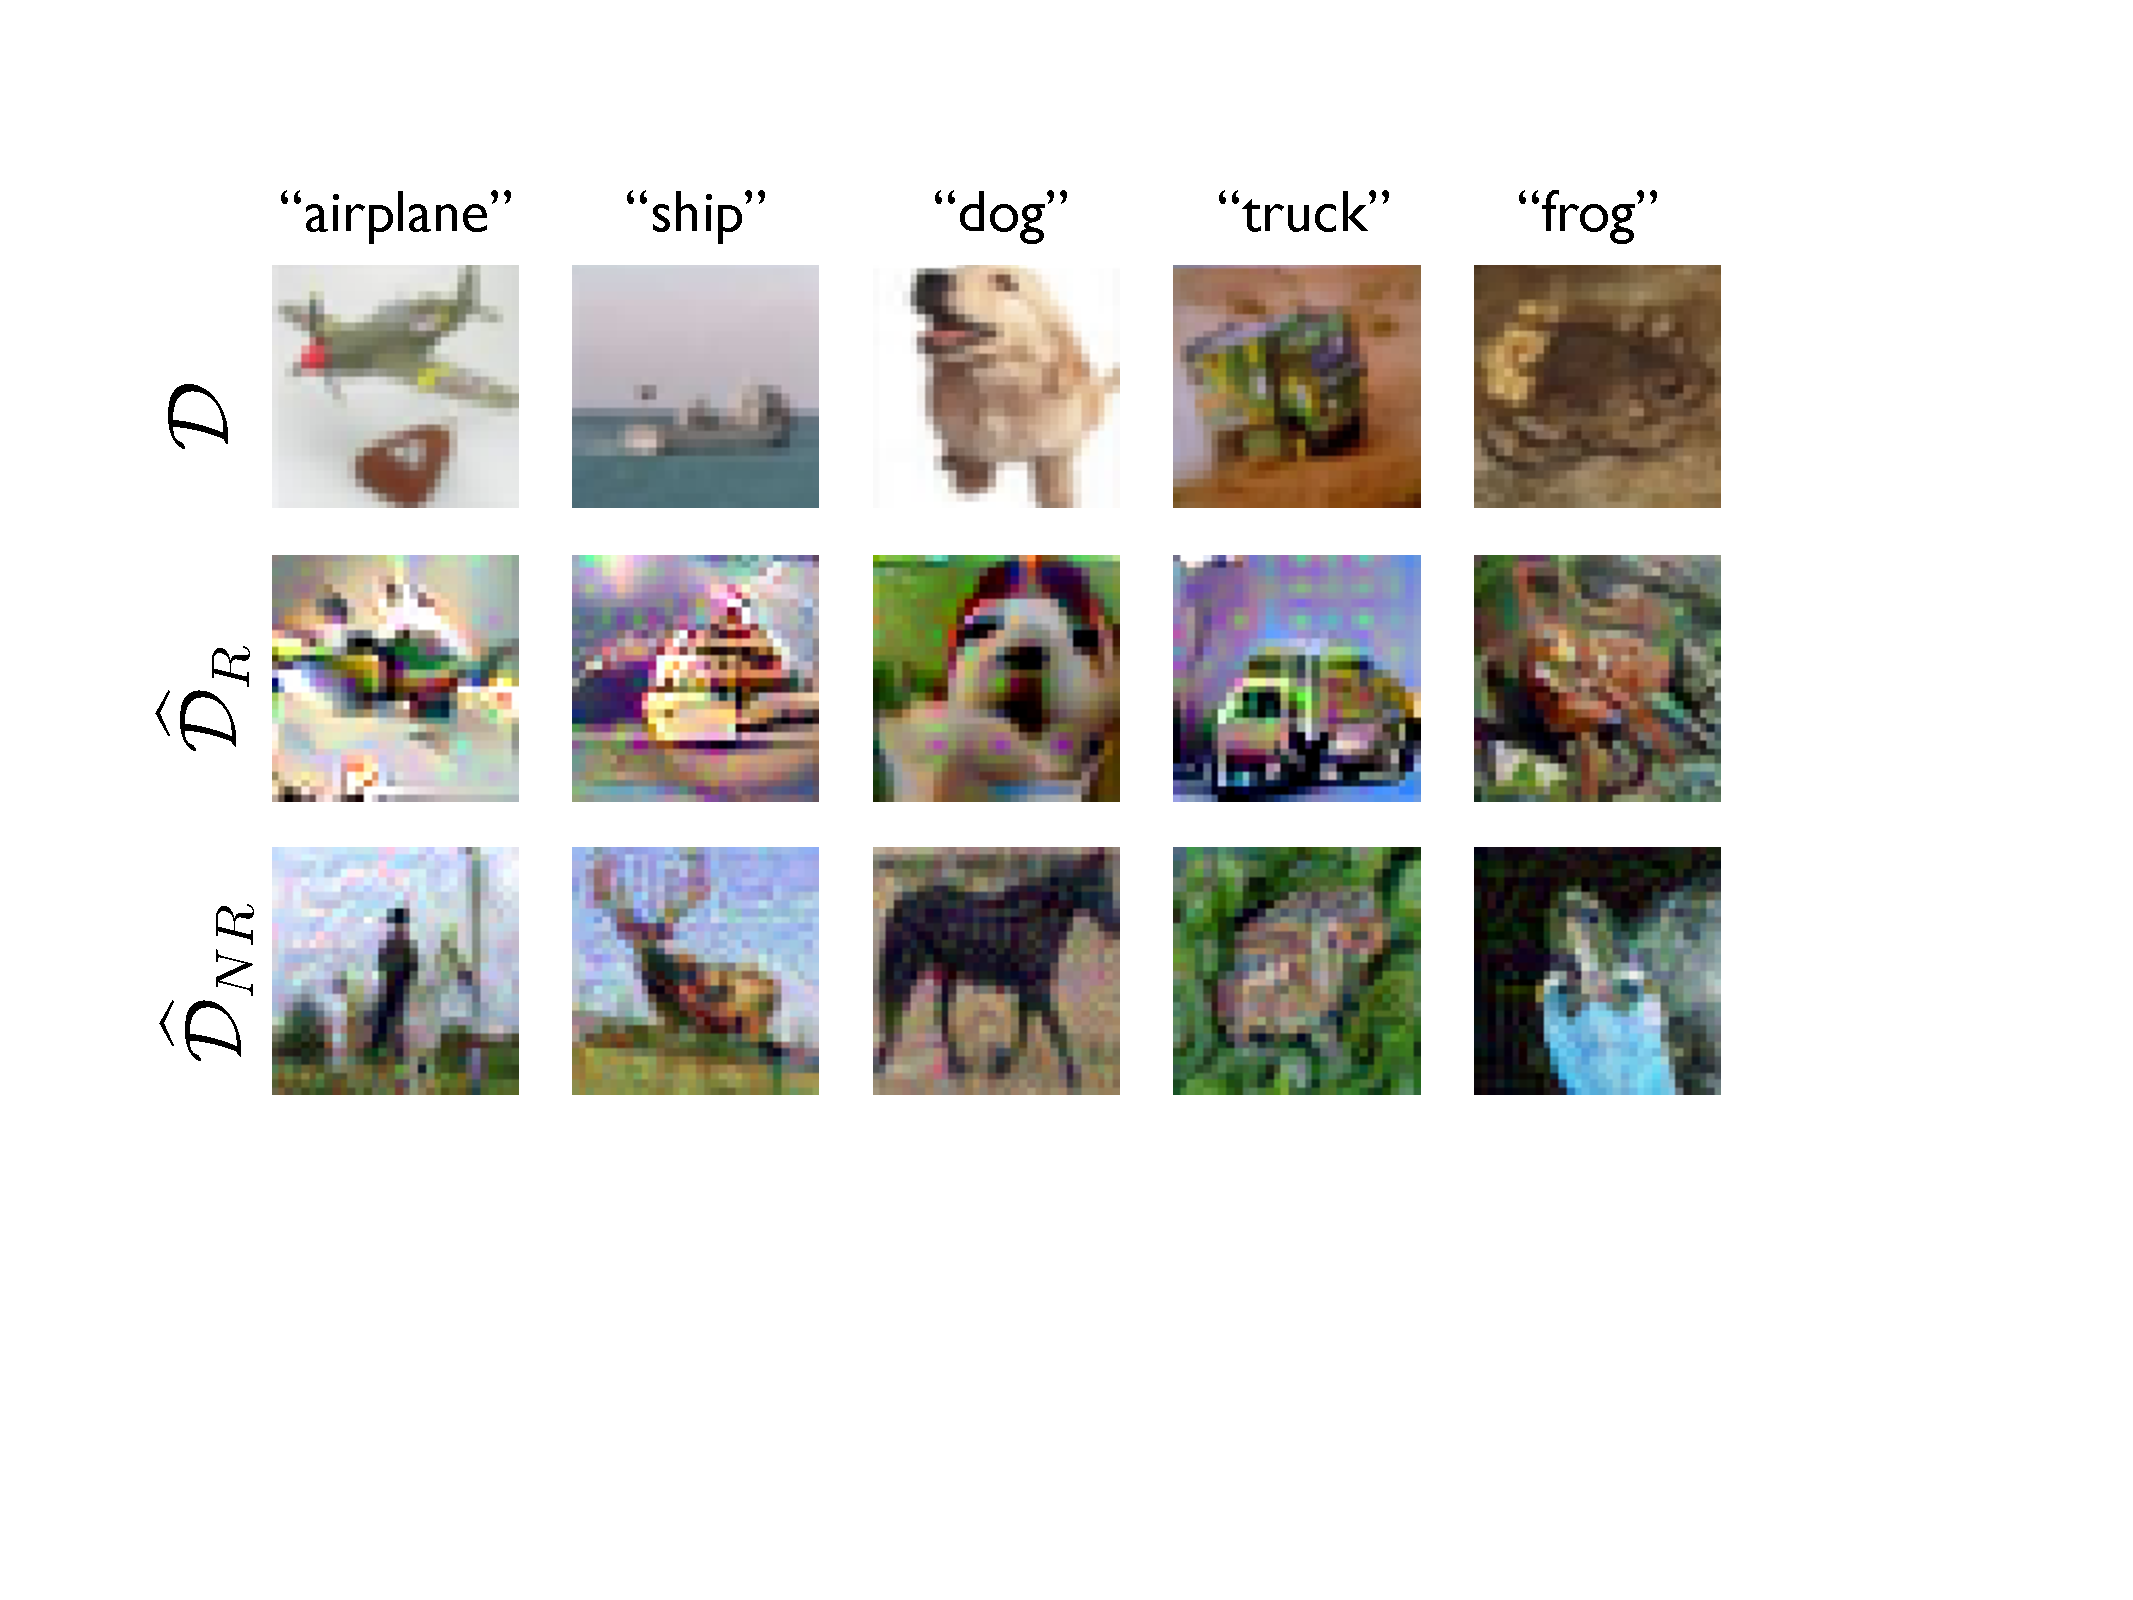
\includegraphics[width=1.0\textwidth]{figures/adversarial-examples/ilyas/cifar_datasets.pdf}
			\caption{}
			\label{fig:robust_inputs}
		\end{subfigure}
		\hfill
		\begin{subfigure}[b]{0.49\textwidth}
			\centering
			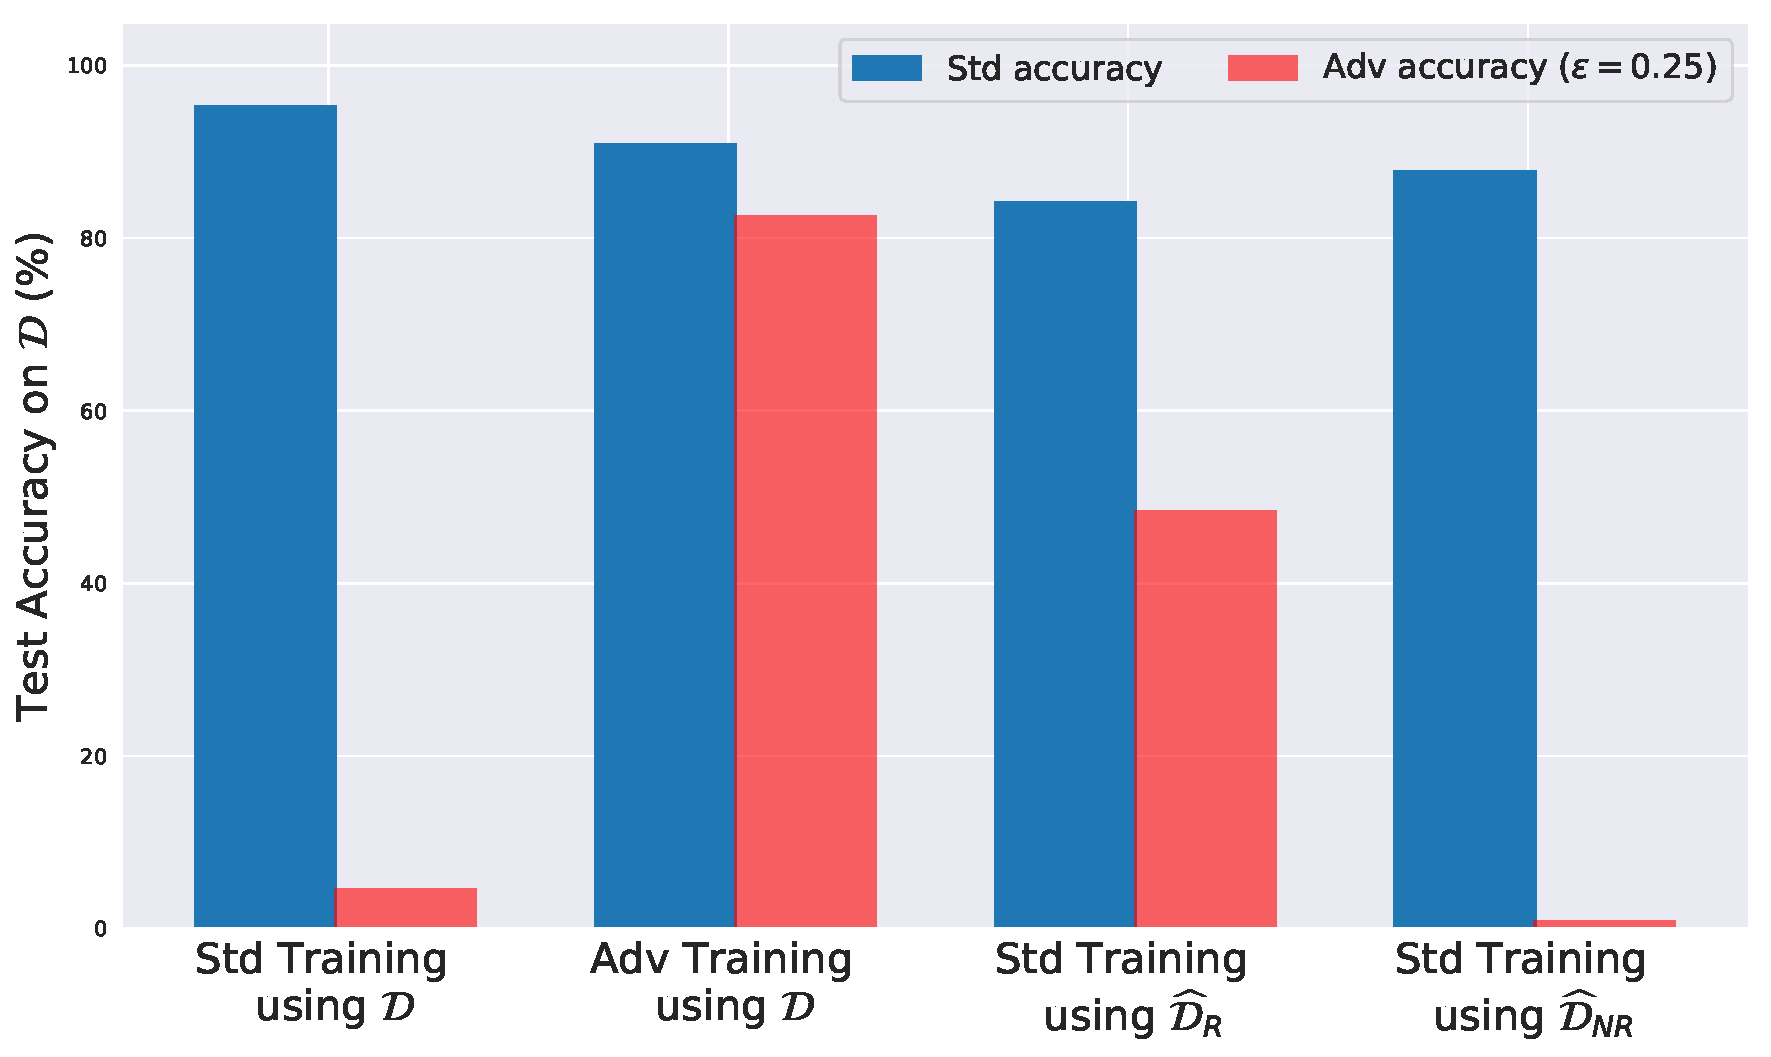
\includegraphics[width=\textwidth]{figures/adversarial-examples/ilyas/CIFAR_res.pdf}
			\caption{}
			\label{fig:robustify_cifar}
		\end{subfigure}
		\caption{
			(a) Random samples from variants of the
			CIFAR-10 training set:
			the \textbf{original} training set; 
			the \textbf{robust training set} $\set D_\text{R}$, with features used by a
			robust model; and
			the \textbf{nonrobust training set} $\set D_\text{NR}$, with
			features relevant to a standard model.
			(b) Standard and robust accuracy on the CIFAR-10
			test set ($\set D$) for models trained with standard training, adversarial training, and standard training on datasets $\set D_\text{R}$ (robust) and $\set D_\text{NR}$ (nonrobust). Adapted from \citet{Ilyas:2019:AENBTF}.}
		\label{fig:iliyas-experiment-results}
	\end{figure}
\end{frame}
\note[itemize]{
	\item\item 0:20 / 10:20
}

\begin{frame}[allowframebreaks=0.9]{Training with on-manifold adversarial examples}
	\begin{itemize}
		\item \citet{Stutz:2018:DARG} challenge the hypothesis that there is a fundamental trade-off between robustness and generalization. 
		
		\item They hypothesize that most adversarial examples come from directions orthogonal to the learned class manifolds and that training with adversarial examples (as per a definition similar to definition \ref{def:ae-consistent}) limited to the known or learned class manifolds (on-manifold adversarial examples) can improve generalization. 
		\item Experiments with a synthetic dataset with known class-invariant transformations and datasets with small images support the hypothesis that generalization can be improved with adversarial training with on-manifold adversarial examples.
	\end{itemize}

	\begin{figure}[htbp!]
		\begin{center}
			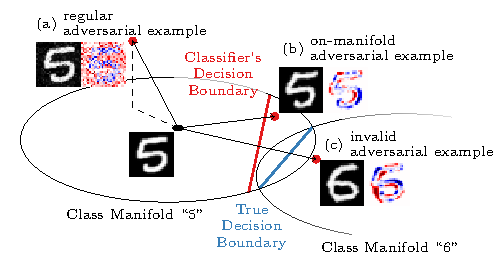
\includegraphics[width=\columnwidth]{figures/adversarial-examples/stutz-introduction_b.pdf}
		\end{center}
		\caption{An illustration by \citet{Stutz:2018:DARG} of class manifolds (classes "5" and "6") with a regular (off-manifold) adversarial example and an on-manifold adversarial example.}
		\label{fig:stutz-illustration}
	\end{figure}
	\begin{itemize}
		\item In one of the experiments \citet{Stutz:2018:DARG} construct a synthetic dataset with a known manifold (geometric transformations of letters) in order to be able to generate exactly on-manifold adversarial examples by modifying parameters of the geometric transformations. With this dataset, they succeed in improving generalization and on-manifold robustness\footnote[frame]{By the authors' definition of an adversarial example, which is similar to the consistent definition (definition \ref{def:ae-consistent}), except for that there is no closeness constraint, making it equivalent to the definition of a misclassified example, on-manifold robustness essentially boils down to generalization.} with adversarial training.
		
		\item In other experiments they use EMNIST \citep{Cohen:2017:EMNIST}, FashionMNIST \citep{Xiao:2017:FMNIDBMLA} and CelebA \citep{Liu:2015:DLFAW}. In order to better approximate class manifolds and disable leaving the manifold of a class when an adversarial example is generated for adversarial training, they first train one variational autoencoder (VAE-GAN) per class. They perform training and evaluation analogously to the experiment with synthetic data by allowing the attack to perturb the latent representation of the autoencoder corresponding to the correct class. They measure positive correlation between robustness to on-manifold adversarial examples and generalization. They observe worse quality of on-manifold adversarial examples for the more complex dataset CelebA due to worse approximation quality of their VAE-GAN-s.
	\end{itemize}
\end{frame}
\note[itemize]{
	\item\item 0:20 / 10:20
}

\section{Conclusion} \label{sec:conclusion}

\begin{frame}[allowframebreaks=0.9]{Conclusion}
	\begin{itemize}
		%\item The existence of adversarial examples shows that common machine learning algorithms ...
		\item Some recent results \citep{Stutz:2018:DARG} suggest that finding ways of improving both robustness generalization might be an interesting research direction to explore.
	\end{itemize}
\end{frame}
\note[itemize]{
	\item\item 0:20 / 10:20
}

\begin{frame}[allowframebreaks=0.9]
	\frametitle{References}
	{\printbibliography}
	%\bibliography{bibliography}
	%\bibliographystyle{apalike}
\end{frame}

\appendix

\appendsubframes


\end{document}
